
\chapter{基于三阶相关相位恢复的彩色成像方法}

透过复杂散射介质或在介质内部的光学成像对于生物医学应用来说是一项艰巨的挑战。其根本问题在于,通过散射介质的光会被强烈散射并扩散成复杂的散斑图案,使物体的颜色和空间信息变得无序混乱\cite{Freund1988,goodman_speckle_2007,bertolotti_non-invasive_2012,katz_non-invasive_2014,Yllmaz2019}。
在散射介质成像的领域中,许多方法已被证明能够克服或利用散射效应\cite{newman_imaging_2016,godara_adaptive_2010,katz_looking_2012,larson_water-soluble_2003,liu_imaging_2011,paniagua-diaz_blind_2019},例如自适应光学\cite{godara_adaptive_2010}、波前整形\cite{katz_looking_2012}、相关成像\cite{bertolotti_non-invasive_2012,katz_non-invasive_2014}、多光子荧光成像\cite{liu_imaging_2011,larson_water-soluble_2003}、鬼成像\cite{paniagua-diaz_blind_2019}和光学相干断层扫描成像\cite{park_full-field_2014}。

同时,通过散射介质进行的彩色成像\cite{conkey_color_2012,leung_acousto-optic_2013,sahoo_single-shot_2017}在对深层组织的非侵入性成像和其他生物医学应用方面扮演着重要的角色,进一步的发展将有利于生物医学应用。随着空间光调制器技术的发展,利用波前整形技术实现了透过散射介质实现彩色成像\cite{leung_acousto-optic_2013,sahoo_single-shot_2017}。
然而,波前整形技术耗时较长,需要对众多像素或者模式进行逐个优化,难以在非入侵的情况下实现波前优化整形。20017年,新加披学者Sahoo等人\cite{sahoo_single-shot_2017}利用光学光谱点扩散函数(Spectral Point Spread Function, sPSF)\cite{Freund1988,goodman_speckle_2007}的去相关性,通过去卷积技术,实现了透过散射介质的彩色成像和光谱成像。
然而,该方法受到光谱去相关带宽的和去卷积计算的限制,仍然存在以下缺点:(\romannum{1})需要对系统的sPSF进行标定;(\romannum{2})成像质量对光学系统稳定性要求极其苛刻。因此,在不标定系统sPSF的情况下,通过传统的彩色成像技术实现散射介质的彩色成像仍然是一个巨大挑战。

在前面章节中,我们对散斑相关成像的方法进行了阐述,并进行了相关实验验证,实验证明了基于光学记忆效应的散斑相关成像方法能够有效的实现对隐藏目标的成像。该方法的核心思想为:通过计算散斑的自相关$I \bigstar I$,移除掉系统PSF的影响,根据维纳辛钦定律进而获得隐藏目标的傅里叶振幅信息。以恢复隐藏目标的傅里叶振幅信息为支撑,利用相位恢复算法进而实现了隐藏目标的的傅里叶相位信息猜测,实现了隐藏目标的成像。
常见的相位恢复算法需要尝试多次的随机初始猜测,才能较好的恢复图像,但是该方法难以保证正确的恢复隐藏目标的方向信息。当所恢复的隐藏目标方向信息不能保证时,对于透过散射散射介质的彩色成像造成了更大困难。我们是否能够找到恰当的相位恢复算法,确定性的恢复目标,进而实现透过散射介质的彩色成像?

在本章中,我们提出了一种基于三阶相关相位恢复的透过散射介质的彩色成像方法。首先,我们证明了三阶相关相位恢复技术的基本理论;其次,我们通过仿真和实验的方式验证了基于三阶相关相位恢复的散射成像有效性;最后,我们通过实验的方式验证了基于三阶相关相位恢复的透过散射介质的彩色成像方法的有效性。与其他相位恢复技术相比,该相位恢复技术可以保留隐藏目标的方位信息,无需额外步骤或更多先验信息去实现透过散射介质的彩色成像。此外,我们的方法有可能实现透过散射介质的光谱成像。

\section{基于三阶相关相位恢复算法的彩色像基本理论}

首先,我们对本章将要进行的彩色成像理论进行简单陈述。该散射成像方法可以简单理解为:即从分别获取RGB三通道的图像,然后合成彩色图像。RGB三通的的图像信息如何获取?我们可以通过彩色相机或者通过添加滤波片的形式进行分别获取。当分别获取RGB通道的散斑后,我们需要分别对单个散斑进行处理,即分别从散斑中获取隐藏目标的傅里叶振幅信息和相位信息。当分别获取恢复RGB通道后的图像后,我们进行相应的图像合成,基本原理如图\ref{fig:4.1}所示。图\ref{fig:4.1}中,$P_1$,$P_2$和$P_3$分别表示所获取的不同通道的散斑,$P_1^{\prime}$,$P_2^{\prime}$和$P_3^{\prime}$表示分别从$P_1$,$P_2$和$P_3$中所恢复的隐藏目标信息。
然后,将$P_1^{\prime}$,$P_2^{\prime}$和$P_3^{\prime}$合成最终的彩色图像$P$。

\begin{figure}[htp]
	\centering
	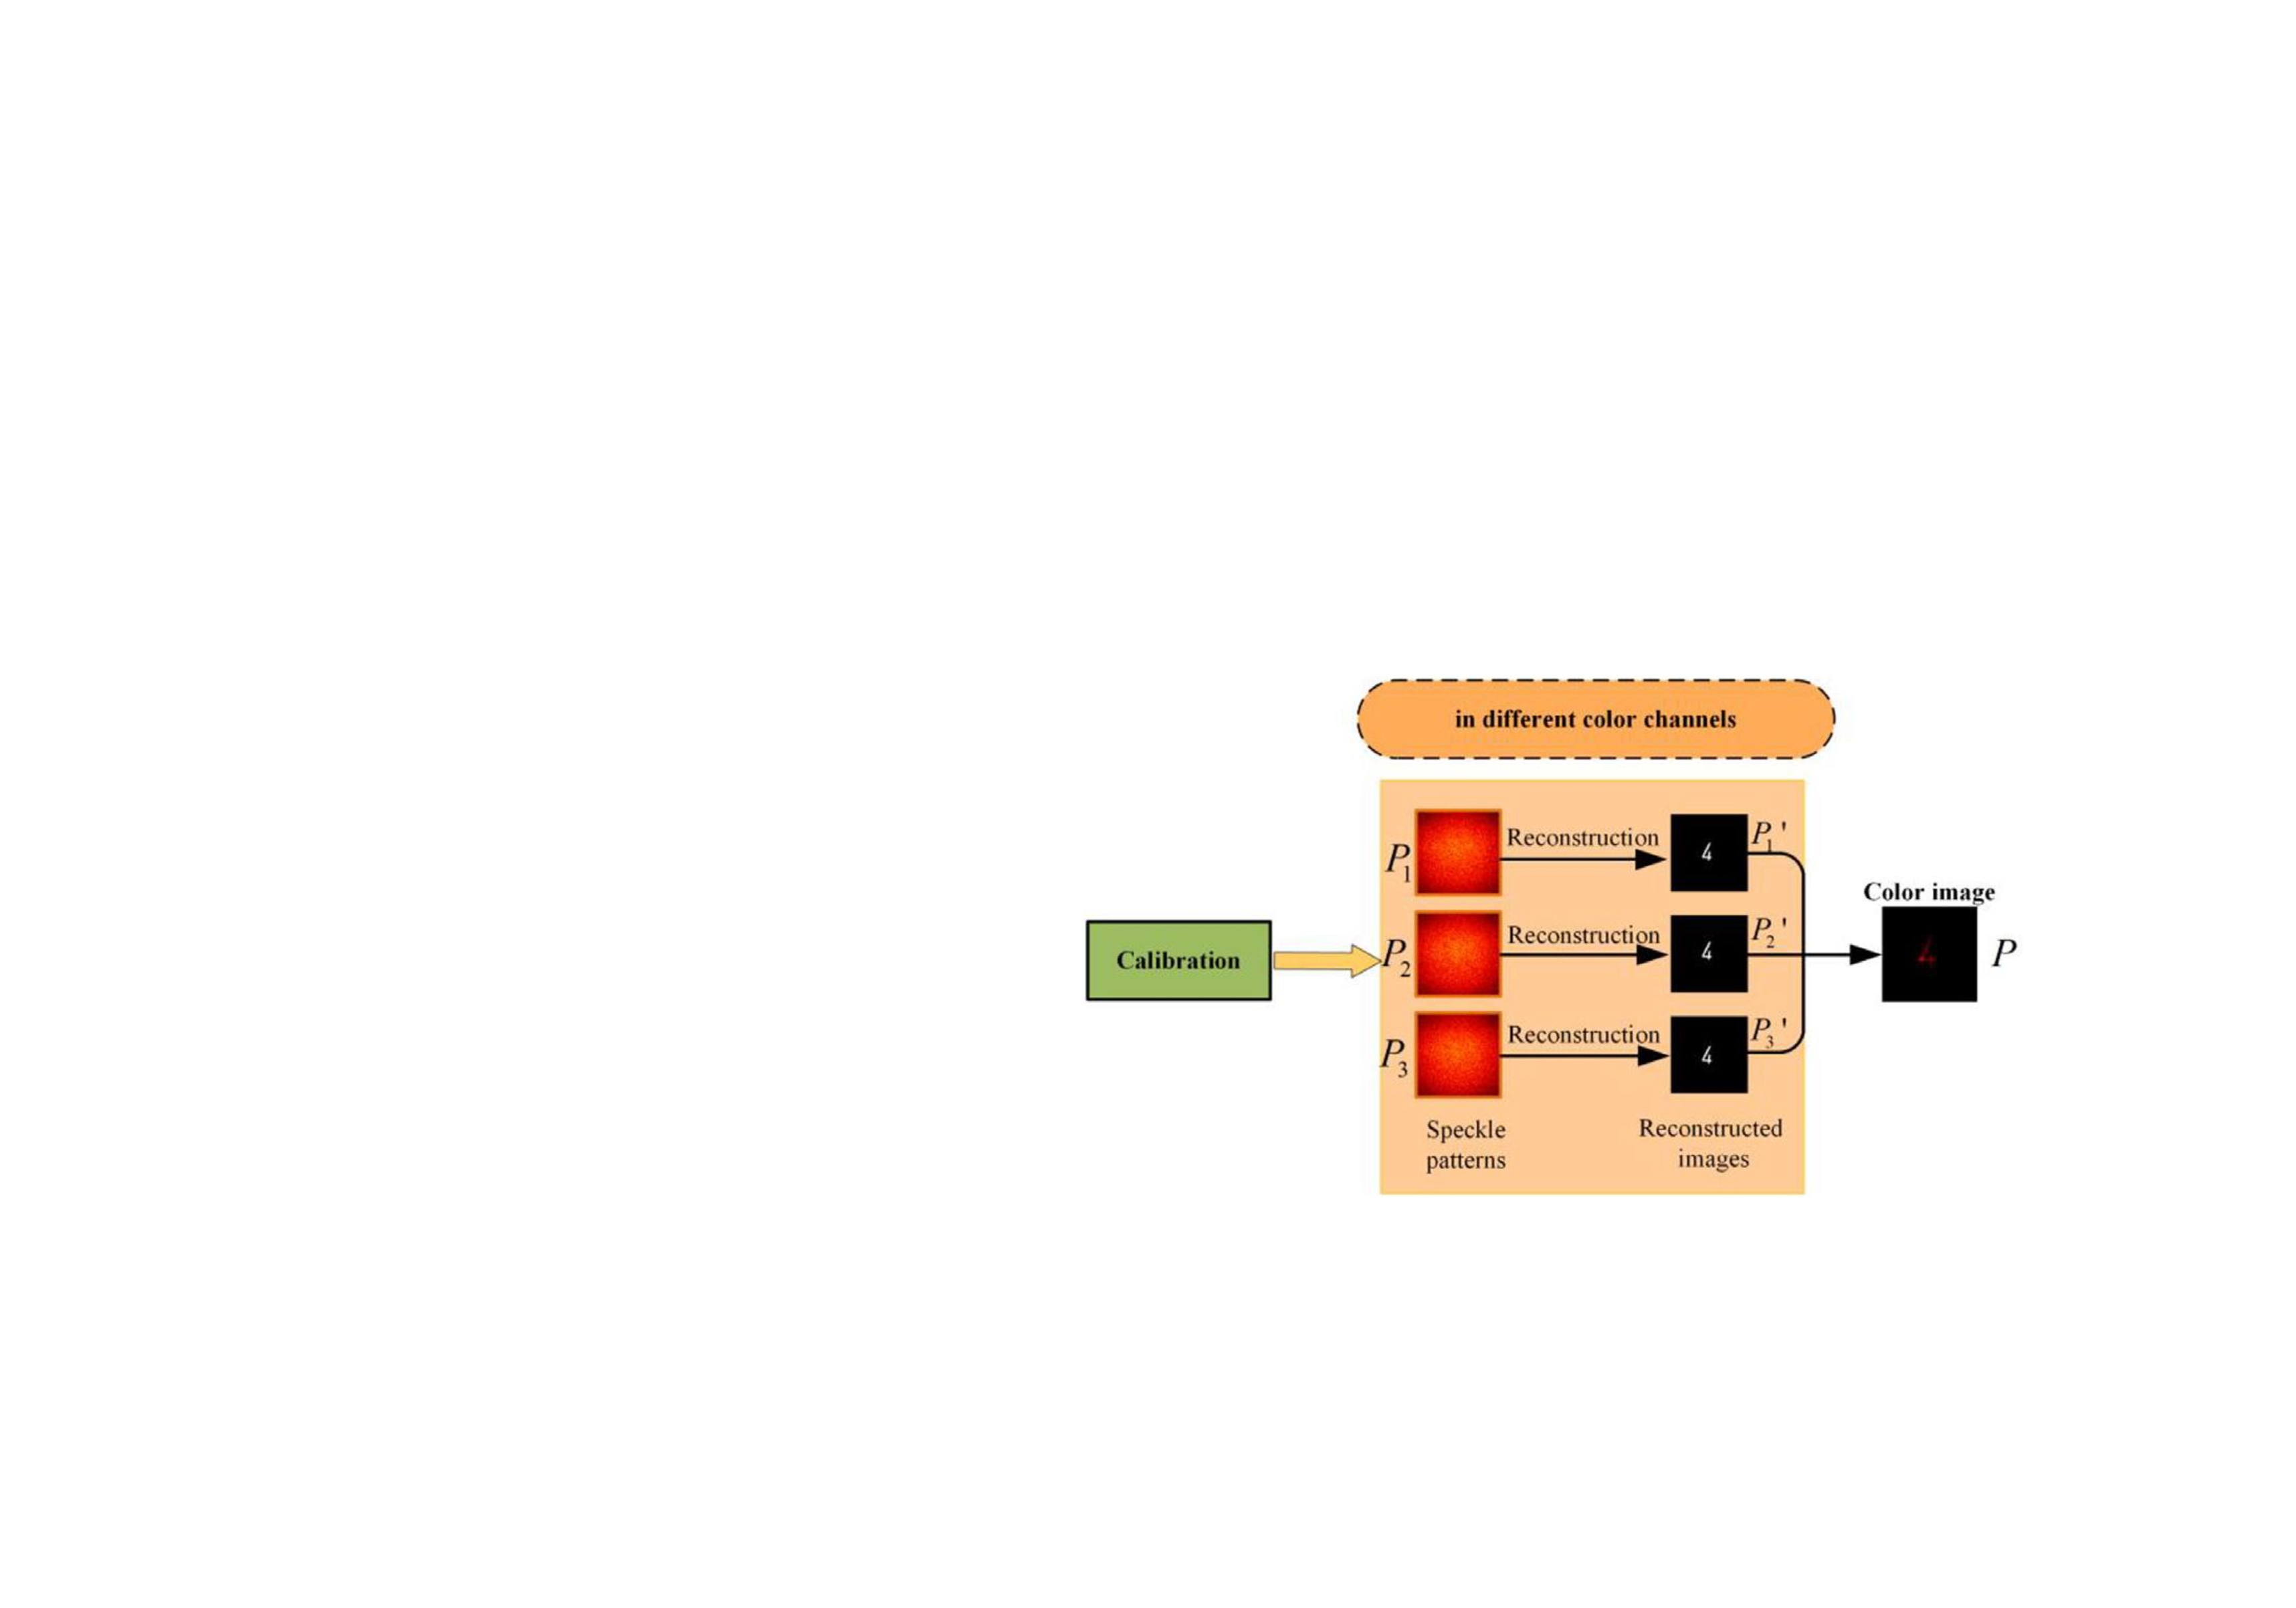
\includegraphics[scale=0.45]{C4.fig1}
	\caption{透过散射介质彩色成像的基本原理}
	\label{fig:4.1}
\end{figure}
在最终合成彩色图像前,如何从单帧散斑中恢复隐藏目标的信息并保存目标的方向信息,如图\ref{fig:4.2}所示,我们将在接下来部分进行详细介绍。
\begin{figure}[htp]
	\centering
	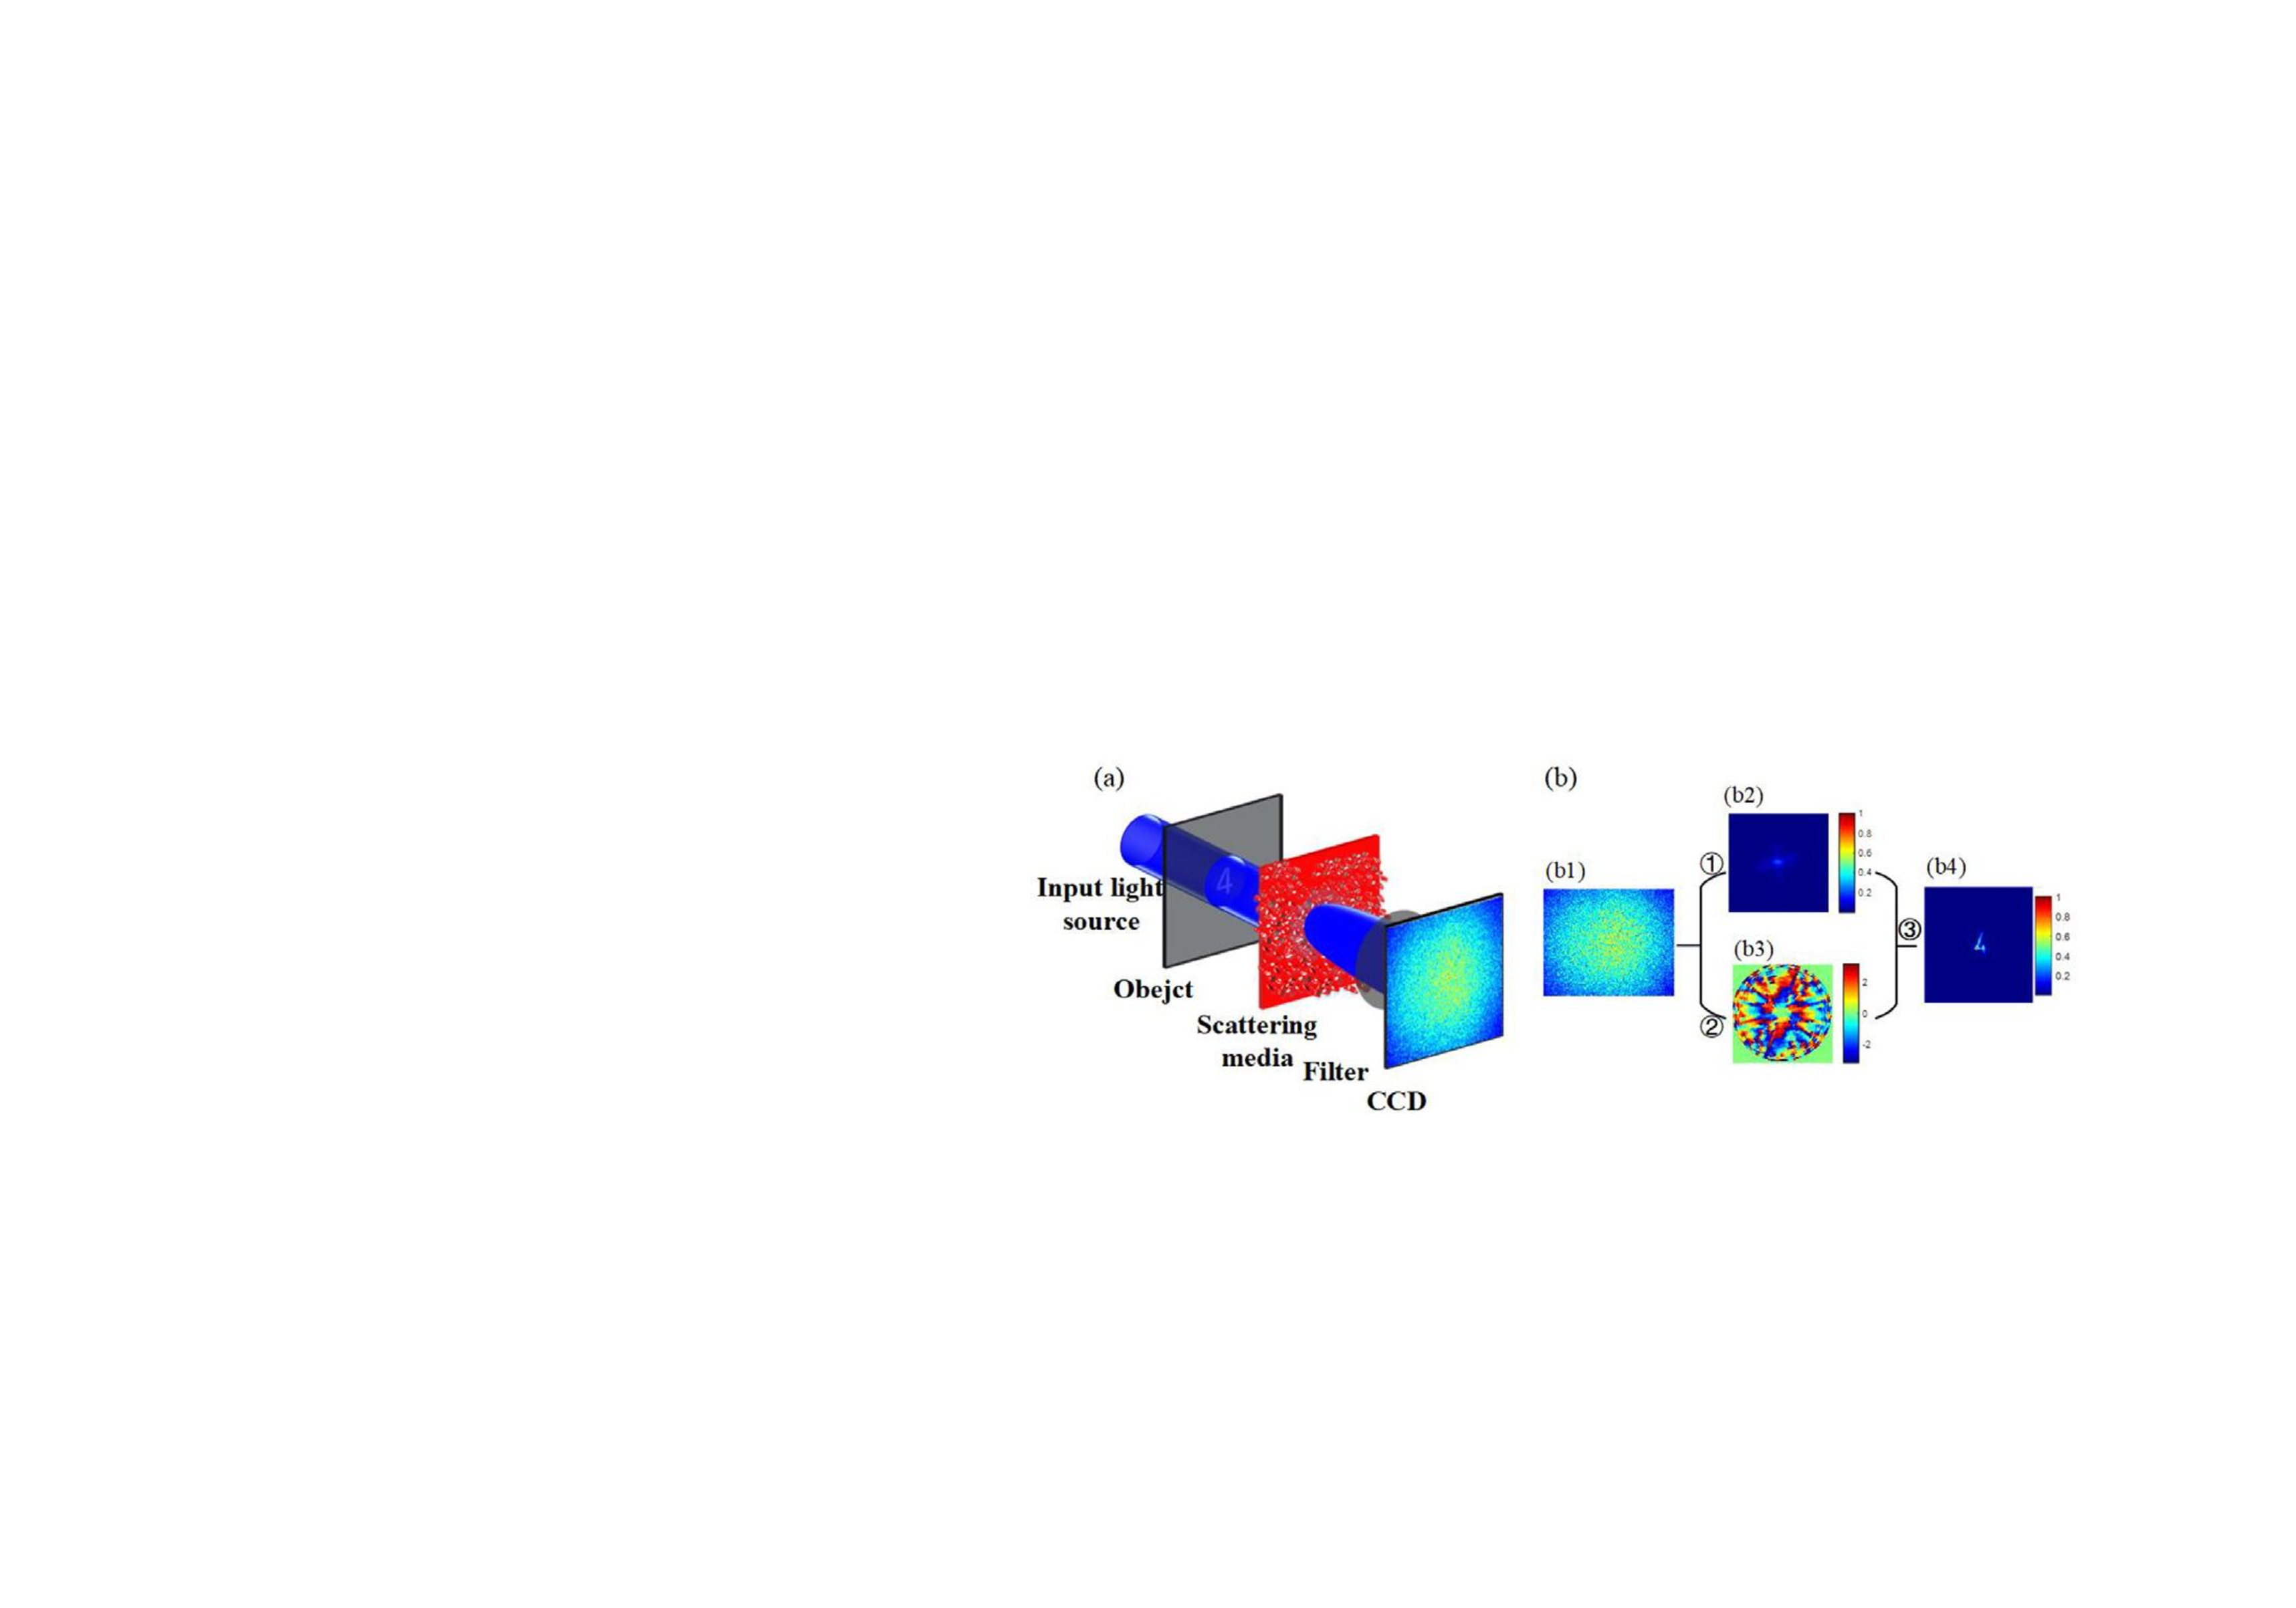
\includegraphics[scale=0.50]{C4.fig2}
	\caption{单帧的透过散射介质成像示意图}
	\label{fig:4.2}
\end{figure}
单帧的透过散射介质成像原理。\ref{fig:4.2}a为实验装置示意图:一束非相干光照亮物体,来自物体的透射光照亮散射介质,最终在CCD上产生散斑图案。\ref{fig:4.2}b为图像恢复流程:(b1)为散斑图案;(b2)为物体的傅立叶振幅; (b3)物体的傅立叶相位和(b4)所恢复的物体。其中,{\large \textcircled{\normalsize 1}}表示自相关过程,{\large \textcircled{\normalsize 2}}表示三阶相关相位恢复过程,{\large \textcircled{\normalsize 3}}表示逆傅立叶变换过程。

\subsection{振幅恢复}
在散射介质光学效应区域内时,系统的PSF具有空间平移不变性,所以系统的成像模型可以卷积形式表示:

\begin{equation}
\begin{aligned}
    I &= (O*S)\\
      &= \iint O(x)*S(x) \mathrm{d}{x}
\end{aligned}
\label{eq:4.1}
\end{equation}
其中,$*$表示卷积符号,$I$表示相机所接收到的散斑强度图像,$O$表示目标和$S$表示系统的PSF。

然后通过计算所获得的相机强度散斑图案的自相关,可以获得目标图案的自相关,如公式(\ref{eq:4.2})所示:

\begin{equation}
\begin{aligned}
    I \bigstar I  &= \iint O(x)*S(x) \mathrm{d}{x} \bigstar \iint O(x)*S(x) \mathrm{d}{x} \\
		              & \cong  (O \bigstar O)
\end{aligned}
\label{eq:4.2}
\end{equation}其中,$\bigstar$表示自相关运算。

根据维纳辛钦定理可知,物体的自相关为其物体的功率谱。因此,我们可以通过傅里叶变换的形式,从物体的自相关中恢复物体的傅里叶振幅信息$\mid \mathcal{F}(O) \mid $,如公式(\ref{eq:4.3})所示:
\begin{equation}
\begin{aligned}
   \mid \mathcal{F}(O) \mid \cong \sqrt{\mathcal{F}(I \bigstar I)}
\end{aligned}
\label{eq:4.3}
\end{equation}其中,$\mathcal{F}$表示傅里叶变换运算。

\subsection{相位恢复}

2016年吴腾飞等人\cite{wu_single-shot_2016}受到天文成像的启发,将三阶相关的相位恢复算法引入到散斑自相关成像技术中,三阶相关的相位恢复算法流程如图\ref{fig:4.3}所示,其中,(a)为散斑图案;(b)为子散斑图案(滤波后);(c)为来自第$m$个子散斑图案的一维信号的三阶相关相位;(d)所恢复物体的最终傅立叶相位。( $\theta$ 表示Radon变换的角度,在(b)和(d)中用红色双箭头标记)。

\begin{figure}[htp]
	\centering
	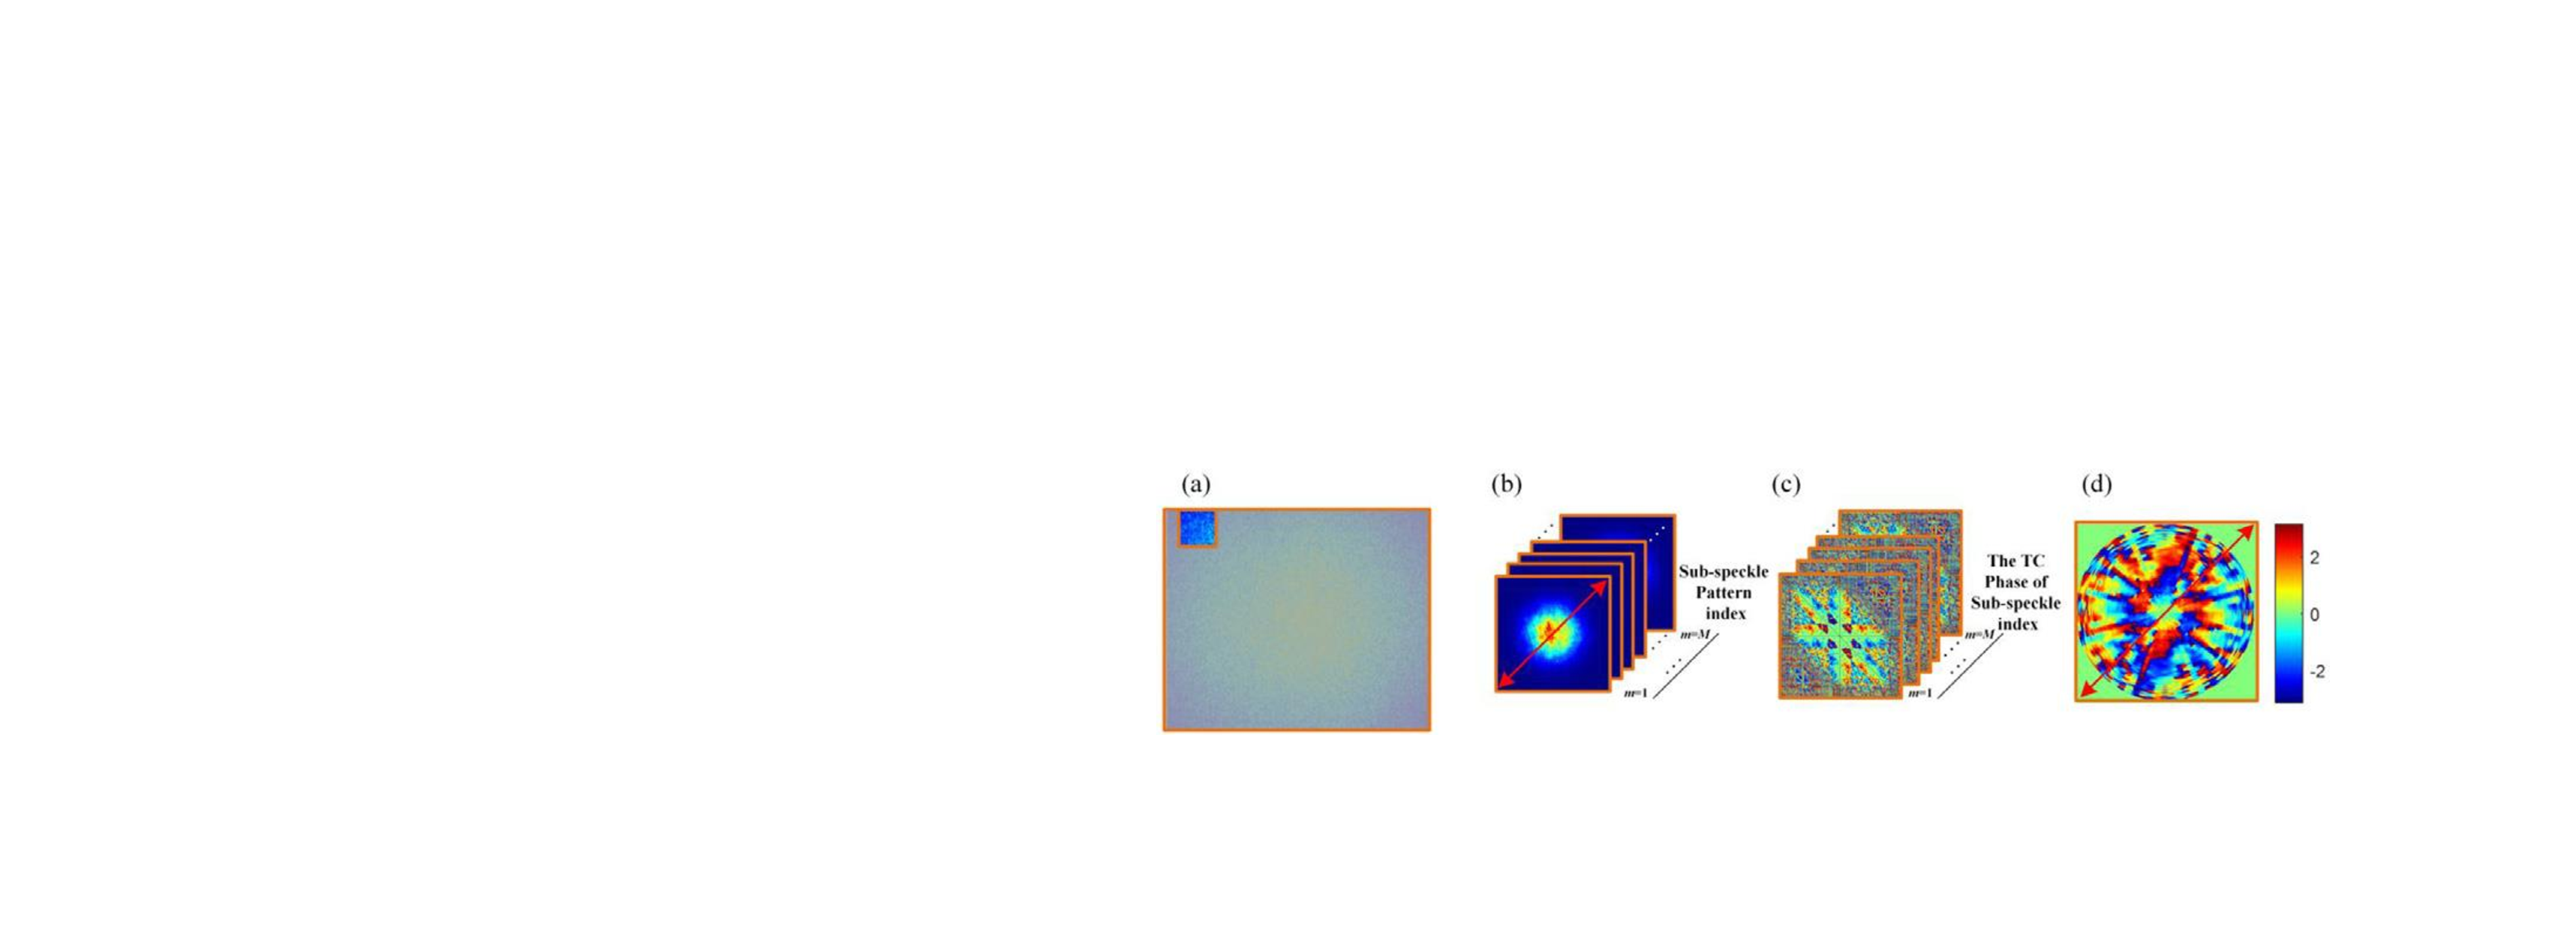
\includegraphics[scale=0.55]{C4.fig3}
	\caption{三阶相关的相位恢复算法流程如图}
	\label{fig:4.3}
\end{figure}

在此相位恢复过程中,隐藏目标的傅立叶相位将从众多子散斑图案中所恢复。首先,我们通过应用 $W_m(x,y)$的方窗函数将散斑图案(\ref{fig:4.3}a)划分为$M$个子散斑图案$I_m(x,y)$(\ref{fig:4.3}b)。其中,每个子散斑图案$I_m(x,y)$具有相同的宽度和高度,统一大小尺寸的子散斑将有助于后期的并行信号处理,且子散斑之间选取重叠区域为$90\%$。

第$m$个子散斑图案$I_m(x,y)$的强度分布可以表示为\cite{goodman_speckle_2007,goodman_introduction_2005}:

\begin{equation}
\begin{aligned}
    I_m = O*S_m
\end{aligned}
\label{eq:4.4}
\end{equation}其中,$O$表示目标的强度分布;$S_m$表示第$m$个子散斑图案所对应的PSF。

在傅里叶空间,公式(\ref{eq:4.5})可以表示为\cite{goodman_speckle_2007,goodman_introduction_2005}:
\begin{equation}
\begin{aligned}
    \mathcal{F} \{ I_m \} = C_m*\mathcal{F}\{ O \}
\end{aligned}
\label{eq:4.5}
\end{equation}其中,$C_m$表示第$m$个子散斑图案所对应系统的光学传递函数(Optical Transfer Function, OTF)。

当目标位于光学记忆效应范围之内时,其成想系统可以看作是为多个点源目标的系统相应函数的非相干叠加\cite{goodman_speckle_2007,goodman_introduction_2005}。因此,该系统的振幅传递函数$H_m$可以展开为两个函数的乘积如公式(\ref{eq:4.6})所示。
\begin{equation}
\begin{aligned}
    H_m = P_m \cdot R_m
\end{aligned}
\label{eq:4.6}
\end{equation}其中,$P_m$表示散射介质所引入的影响,$R_m$表示光瞳函数所引入的影响。在此我们假设$R_m$为一个平稳的随机变量。

同时,OTF$C_m$是振幅传递函数$H_m$的归一化自相关,即:
\begin{equation}
\begin{aligned}
    C_m(\mu) &= \frac{\int{H_m(\mu) \cdot H_m^{*}(\mu + \mu^{\prime})}\mathrm{d}{\mu^{\prime}}}{\iint{|H_m(\mu^{\prime})|^2}\mathrm{d}{\mu^{\prime}}}\\
    &=\frac{\int{P_m(\mu) \cdot P_m^{*}(\mu + \mu^{\prime})} \cdot {R_m(\mu) \cdot R_m^{*}(\mu + \mu^{\prime})} \mathrm{d}{\mu^{\prime}}}{\iint{|P_m(\mu) \cdot P_m^{*}(\mu + \mu^{\prime})} \cdot {R_m(\mu) \cdot R_m^{*}(\mu + \mu^{\prime})}|^2 \mathrm{d}{\mu^{\prime}}}
\end{aligned}
\label{eq:4.7}
\end{equation}

根据三阶相关理论\cite{lohmann_speckle_1983,northcott_algorithms_1988},公式(\ref{eq:4.5})可以表示为:

\begin{equation}
\begin{aligned}
    \mathcal{F} \{ I_m \}^{(3)} = C_m^{(3)}*\mathcal{F}\{ O \}^{(3)}
\end{aligned}
\label{eq:4.8}
\end{equation}其中,$^{(3)}$表示三阶相关运算。

\section{学位论文的版面设置要求}

(1)行间距:固定值~20~磅(题名页除外)。

(2)字符间距:标准。

(3)页眉设置:单面页码页眉标题为章节题目,每一章节的起始页必须在单面页码,双面页码页眉标题统一为“西安电子科技大学博/硕士学位论文”,页眉标题居中排列,字体为宋体,字号为五号。页眉文字下添加双横线,双横线宽度为~0.5~磅,距正文距离为:上下各~1~磅,左右各~4~磅。

(4)页码设置:学位论文的前置部分和主体部分分开设置页码,前置部分的页码用罗马数字标识,字体为~Times New Roman~,字号为小五号;主体部分的页码用阿拉伯数字标识,字体为宋体,字号为小五号。页码统一居于页面底端中部,不加任何修饰。

(5)页面设置:为了便于装订,要求每页纸的四周留有足够的空白边缘,其中页边距为上~3~厘米、下~2~厘米;内侧~2.5~厘米、外侧~2.5~厘米;装订线为~0.5~厘米;页眉~2~厘米,页脚~1.75~厘米。

\section{学位论文的打印、装订要求}

(1)打印:学位论文必须用~A4~纸页面排版,双面打印;

(2)装订:依次按照中文题名页、英文题名页、声明、摘要、插图索引、表格索引、符号对照表、缩略语对照表、目录、正文、附录(可选)、参考文献、致谢、作者简介的顺序,用学校统一印制的学位论文封面装订成册。盲审论文必须删除致谢部分的文字内容(致谢标题须保留)以及封面和研究成果中的作者和指导教师姓名,研究成果列表中应体现作者的排序,如第一作者、第一发明人等。

\section{其他说明}

本规定由研究生院负责解释,从申请~2015~年~9~月毕业和授位的研究生开始执行,其它有关规定同时废止。研究生毕业论文撰写要求参照学位论文撰写要求执行。
